\documentclass[11pt]{book}

\usepackage[ruled,vlined]{algorithm2e}
\usepackage[utf8]{inputenc}

\usepackage{graphicx} 
\usepackage{amsfonts}
\usepackage{amssymb}
\usepackage{amsmath}

\usepackage[pdftex]{color, hyperref}
\hypersetup{colorlinks,%
	citecolor=black,%
	filecolor=black,%
	linkcolor=black,%
	urlcolor=black,%
}
\pdfpagewidth=\paperwidth
\pdfpageheight=\paperheight

% package `subfigure` and `subfig` are deprecated and should not be used
% unless withing the IEEETran or ACM SIG templates
\usepackage{subcaption}

% To handle the acronyms nicely
\usepackage[nonumberlist, toc, acronym]{glossaries}
\newacronym{csma}{CSMA}{Carrier Sense Multiple Access}
\newacronym{fdd}{FDD}{Frequency Division Duplexing}
\newacronym{tdd}{TDD}{Time Division Duplexing}
\newacronym{fdma}{FDMA}{Frequency Division Multiple Access}
\newacronym{tdma}{TDMA}{Time Division Multiple Access}
\newacronym{cdma}{CDMA}{Code Division Multiple Access}
\newacronym{wcdma}{WCDMA}{Wide-band Code Division Multiple Access}
\newacronym{ss}{SS}{Spread Spectrum}
\newacronym{sdma}{SDMA}{Space Division Multiple Access}
\newacronym{ofdm}{OFDM}{Orthogonal Frequency Division Multiplexing}
\newacronym{ofdma}{OFDMA}{Orthogonal Frequency Division Multiple Access}
\newacronym{ufr}{UFR}{Universal Frequency Reuse}
\newacronym{4g}{4G}{4$^{th}$ Generation of Mobile Communications}
\newacronym{3g}{3G}{3$^{rd}$ Generation of Mobile Communications}
\newacronym{3gpp}{3GPP}{3$^{rd}$ Generation Partnership Project}
\newacronym{hspa+}{HSPA+}{High-Speed Packet Access Plus}
\newacronym{lte}{LTE}{Long Term Evolution}
\newacronym{ltea}{LTE-A}{Long Term Evolution Advanced}
\newacronym{mimo}{MIMO}{Multiple Input Multiple Output}
\newacronym{itu}{ITU}{International Telecommunication Union}
\newacronym{itur}{ITU-R}{International Telecommunication Union Radiocommunication Sector}
\newacronym{imta}{IMT-Advanced}{International Mobile Telecommunications-Advanced}
\newacronym{ca}{CA}{Carrier Aggregation}
\newacronym{rn}{RN}{Relay Node}
\newacronym{comp}{CoMP}{Coordinated Multi Point}

\makeglossaries

% To handle the references
\usepackage{natbib}

%%%%%%%%%%%%%%%%%%%%%%%%%%%%%%%%%%%%%%%%%%%%%%%%%%%%%%%%%%%%%%%%%%%%%%%%%%%%%%%%
\newcommand{\refs}[1]{Section~\ref{#1}}
\newcommand{\refss}[1]{Subsection~\ref{#1}}
\newcommand{\reff}[1]{Figure~\ref{#1}}

%%%%%%%%%%%%%%%%%%%%%%%%%%%%%%%%%%%%%%%%%%%%%%%%%%%%%%%%%%%%%%%%%%%%%%%%%%%%%%%%
% Margins
%\setlength{\textheight}{22cm}
%\setlength{\headsep}{1cm}
%\setlength{\topmargin}{-0.5cm}
%\setlength{\textwidth}{14cm}
\setlength{\oddsidemargin}{2cm}
\setlength{\evensidemargin}{2cm}

% Include up to subsections in the TOC
\setcounter{tocdepth}{3}

% So that the empty pages have no page number
\makeatletter
  \def\cleardoublepage{\clearpage\if@twoside \ifodd\c@page\else
  \vspace*{\fill}
    \thispagestyle{empty}
    \newpage
    \if@twocolumn\hbox{}\newpage\fi\fi\fi}
\makeatother

%%%%%%%%%%%%%%%%%%%%%%%%%%%%%%%%%%%%%%%%%%%%%%%%%%%%%%%%%%%%%%%%%%%%%%%%%%%%%%%%
% PREFACE
%%%%%%%%%%%%%%%%%%%%%%%%%%%%%%%%%%%%%%%%%%%%%%%%%%%%%%%%%%%%%%%%%%%%%%%%%%%%%%%%
\begin{document}

% \frontmatter
% % First part uses roman numbering
\pagenumbering{gobble}
% \cleardoublepage
% {\Large

% \begin{figure}[t]
% 	\centering
% 	\centerline{  
% 	
\includegraphics[width=3.5cm]{./ch0/logo.uc3mGrande.eps} 
% 	} 
% \end{figure}


\centerline{UNIVERSIDAD CARLOS III DE MADRID}

\centerline{Departamento de Teoría de la Señal y Comunicaciones}


\vspace*{2.5cm}
\centerline{DOCTORAL THESIS}

\vspace*{1cm}
\begin{center}
{\bf
	BLOCK DIAGONALIZATION TECHNIQUES FOR CELLULAR NETWORKS: CLUSTERING AND SCHEDULING
}
\end{center}

\vspace*{3cm}
Author: JUAN JOSÉ GARCÍA FERNÁNDEZ

Advisor: ANA GARCÍA ARMADA

Date: TBD (Hopefully not far from now)

} % Large

% \newpage
% 
% \cleardoublepage
% \begin{tabular}{l l}
{\bf Tesis Doctoral:} 
& BLOCK DIAGONALIZATION TECHNIQUES\\
& FOR CELLULAR NETWORKS:\\
& CLUSTERING AND SCHEDULING\\
\\
{\bf Autor:} 
& Juan José García Fernández\\
\\
{\bf Director:} 
& Dra. Ana García Armada
\\
\end{tabular}


\vspace*{2cm}

{\large El tribunal nombrado para juzgar la tesis doctoral arriba citada, compuesto por los doctores}


\vspace*{1cm}

Presidente:

\vspace*{2cm}

Vocal:


\vspace*{2cm}

Secretario:

\vspace{2cm}
{\large acuerda otorgarle la calificación de}

\vspace{2cm}
{\large Leganés, a}

% \newpage
% 
% \cleardoublepage
% {\Huge {\bf Acknowledgements}}

\lipsum[5]

% \newpage
% 
% \cleardoublepage
% \pagenumbering{Roman}
% {\Huge {\bf Abstract}}

\lipsum[5]

% \newpage
% 
% \cleardoublepage
% {\Huge {\bf Resumen}}

\lipsum[5]

% \newpage

% Index
\tableofcontents{}

% List of tables and Figures
% \addcontentsline{toc}{chapter}{\protect\numberline{}{Lista de tablas}}
\listoftables{}
\listoffigures{}

% Acronyms
\printglossary[type=\acronymtype]

\mainmatter
%%%%%%%%%%%%%%%%%%%%%%%%%%%%%%%%%%%%%%%%%%%%%%%%%%%%%%%%%%%%%%%%%%%%%%%%%%%%%%%%
% CHAPTERS
%%%%%%%%%%%%%%%%%%%%%%%%%%%%%%%%%%%%%%%%%%%%%%%%%%%%%%%%%%%%%%%%%%%%%%%%%%%%%%%%

% % Back to arabic numbering
% \pagenumbering{arabic}

% Introduction
\chapter{Introduction}\label{ch:intro}

Every new generation of cellular network technologies comes with a new set of
requirements, dictated by the trends in the use of the mobile connectivity. A
common requirement to every single generation is their striving for higher data
rates and greater power efficiency. This motivates research and techology
innovation in order to achieve the goals set for each generation.


The research associated usually requires revisiting old paradigms used in
previous generations, and updating them with novel ideas.


The \emph{release 7} of the \gls{3gpp} \gls{3g} specifications \citep{3Grel7},
also known as \gls{hspa+}, inluded the use of \gls{mimo} as a means to increase
the rates of transmission.


\emph{Release 8}, more well known by its commercial name \gls{lte} \citep{3gpplte},
introduced a new physical layer, based on \gls{ofdm} instead of \gls{wcdma} as in
\gls{3g}. Although the rates attainable with \gls{wcdma} may be comparable to those
obtained with \gls{ofdm}, the latter provides a much easier equalization mechanism
that makes dealing with multipath channels a simpler task. Apart from that \gls{ofdm}
provides a higher flexibility in the resource allocation and user and enables the
use of \gls{ofdma}.

\gls{lte} did not meet the requirements issued by the \gls{itur} \gls{imta} radio
interface \citep{imta} for what is known as \gls{4g} though.

The introduction of \gls{ltea} in \emph{release 10} of the LTE specification
\citep{3gppltea} met the requirements to be considered an \gls{imta} system. The main
novelties included in \gls{ltea} are \gls{ca}, enhanced use of MIMO techniques and support
for \gls{rn}.

\emph{Release 11} \citep{lterel11} included in the specification the support for
\gls{comp} operation. \gls{comp} was included in order to improve the network
performance at cell edges, for it uses several transmitters to provide coordinated
transmission in the downlink, and a number of receivers to provide coordinated
reception in the uplink.

The \gls{comp} operation considered in \citep{lterel11} is just a part of a much
broader field of multi-cell cooperation or coordinated communications where several
cells are assumed to cooperate, in the sense that they take measures in order to
alleviate to a certain degree the level of interference introduced into other parts
of the network, or the use of that interference to their advantage.

\begin{figure}[t]
    \centering
    \begin{subfigure}[b]{0.45\textwidth}
        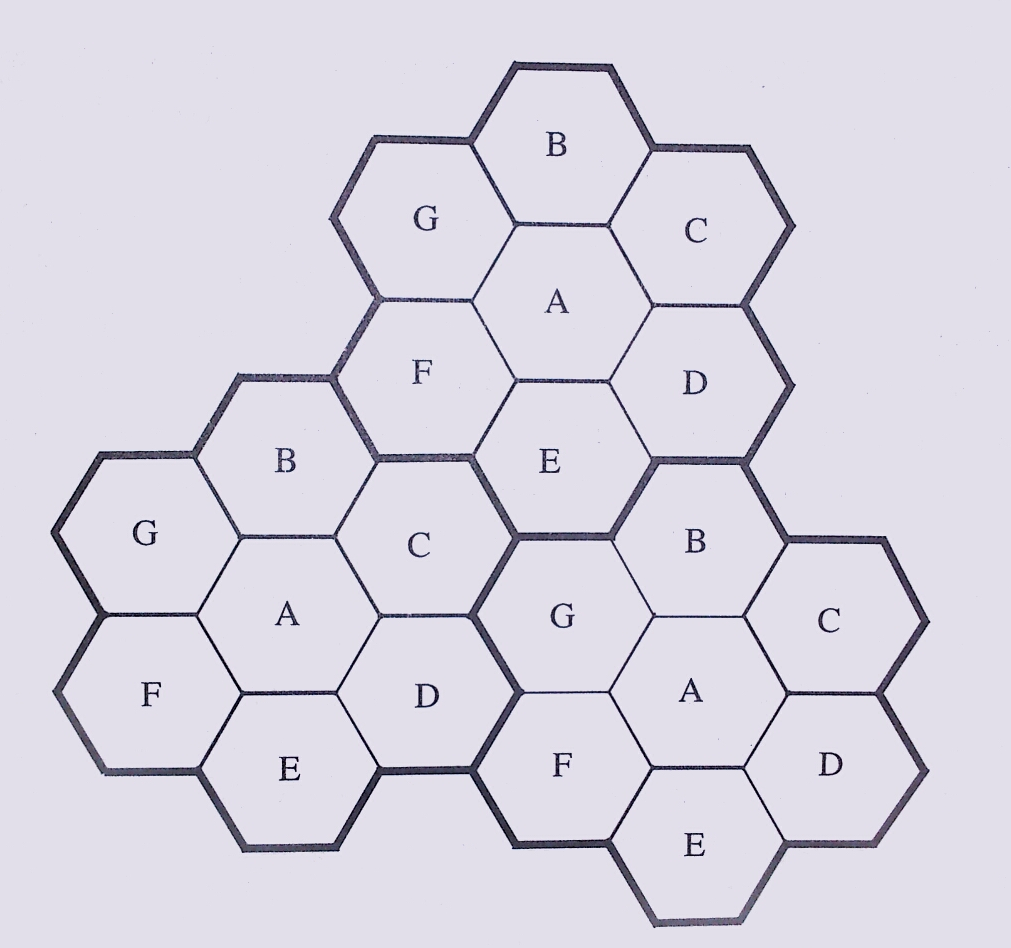
\includegraphics[width=\textwidth]{./ch1/img/frequency_reuse.png}
        \caption{Frequency reuse factor of $1 / 7$.}
        \label{fig:freuse}
    \end{subfigure}
    % Comment out the line break that is introduced with the blank line
    % so that it does not put the images one on top of the other...
    \begin{subfigure}[b]{0.45\textwidth}
        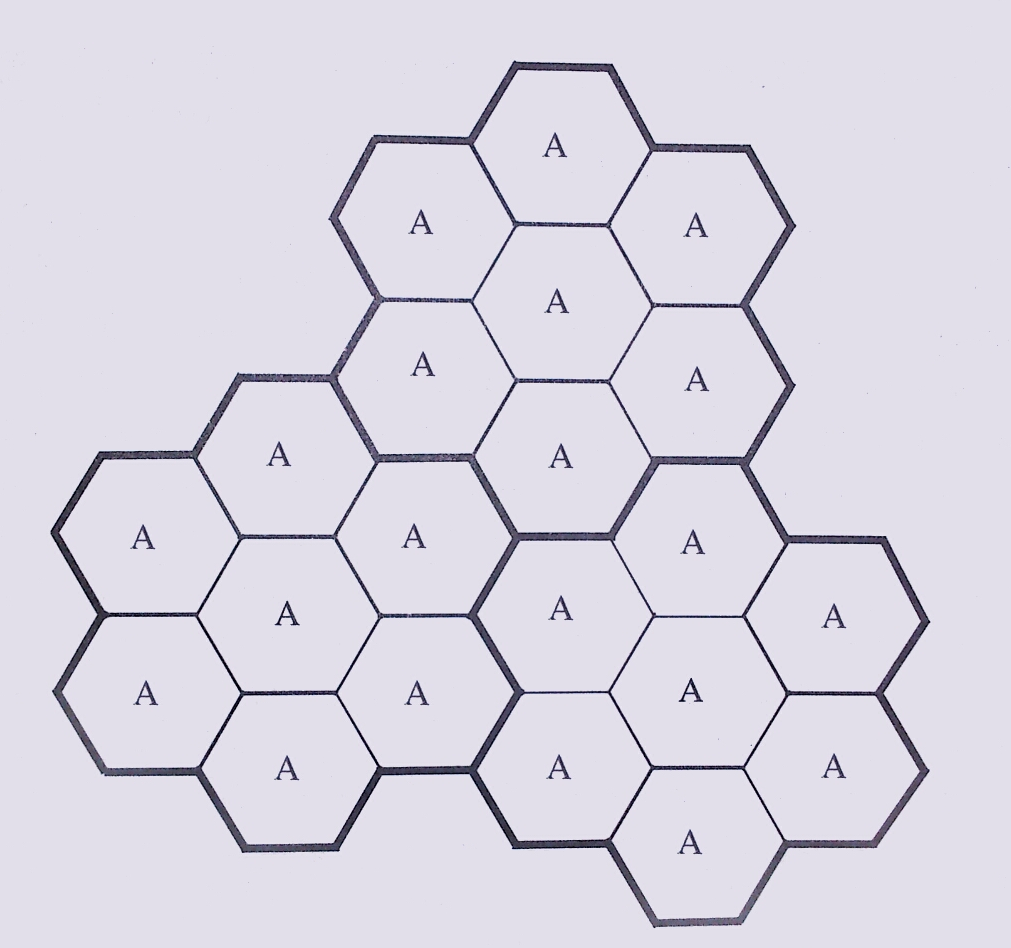
\includegraphics[width=\textwidth]{./ch1/img/universal_freq_reuse.png}
        \caption{Frequency reuse factor of $1$.}
        \label{fig:ufreuse}
    \end{subfigure}
    \caption{Different frequency planning options}
\end{figure}

In the search for higher spectral data rates and a more efficient use of the
resources, \gls{ufr} arises as an alternative in order to make the most out of
the scarce resource that the radio frequency spectrum is. The conventional approach
for cellular networks was to perform a careful frequency planning in order to
avoide the interference among neighboring cells. Clusters of $N$ cells were grouped
together, and assigned $N$ frequency bands to be used, and the pattern is repeated
for different clusters, yielding what is called a \emph{frequency reuse factor}
of $1 / N$, as exemplified in \reff{fig:freuse}.

The problem that this poses is that the available spectrum must be split, which
is an inherent inefficiency in the use of the resources.

\gls{ufr}, in turn, implies that neighboring cells share a common spectrum, as it
can be seen in \reff{fig:ufreuse}, which means that they would be interfering each
other. Therefore, "A new look at the interference" \citep{gesbert10} is needed.

In multi-cell cooperative communications, multiple cells are assumed to cooperate,
in the sense that they take measures in order to alleviate to a certain degree the
level of interference introduced into other parts of the network, or to use that
interference to their advantage. The conventional concept of the interference as
being an impairment shifts to a new point of view where the interference can be
used to improve the overall performance of the network.


% State of the art

% System Model - Block Diagonalization

% Clustering Analysis

% Scheduling

% Conclusions


%%%%%%%%%%%%%%%%%%%%%%%%%%%%%%%%%%%%%%%%%%%%%%%%%%%%%%%%%%%%%%%%%%%%%%%%%%%%%%%%
% REFERENCES
%%%%%%%%%%%%%%%%%%%%%%%%%%%%%%%%%%%%%%%%%%%%%%%%%%%%%%%%%%%%%%%%%%%%%%%%%%%%%%%%
\addcontentsline{toc}{chapter}{\protect\numberline{}{References}}
\bibliographystyle{abbrvnat}
\bibliography{./bibliography/references} 

\end{document}
